\chapter{Estado del arte}

\section{TMSs y su importancia en la logística}
Gracias al artículo \textcite{comparativaSistemasTMS} podemos ver las ventajas y desventajas de los principales TMSs del mercado.
Un sistema TMS (\textit{Transportation Management System}) es una herramienta que permite a las empresas gestionar de manera eficienta el transporte de mercancias. Las funcionalidades más comunes en estos sistemas son
la planificación de rutas, seguimiento de envíos en tiempo real, gestión de proveedores y control de costes.

Según el \textcite{keyAttributesChallengesAndSuccessFactors}  en empresas 3LP (dedicadas al servicio de logística para terceros) el éxito se radica en la satisfacción del cliente, para ello que estas empresas cuenten con TMSs que satisfagan todas las necesidades del negocio es de vital importancia ya que se traduce en entregas de a tiempo, de manera correcta y con total transparencia. Por lo tanto estos sistemas dotan a la empresa de:
\begin{itemize}
    \item Mayor satisfacción del cliente.
    \item Mejora en sostenibilidad de la cadena de suministro.
    \item Tomas de decisiones más rápidas y precisas.
    \item Optimización de modelos de negocio y procesos.
\end{itemize}

\section{Principales proveedores de sistemas TMS en el mercado}

\begin{enumerate}
    \item \textbf{Oracle Transportation Management (OTM):} Aplicación más completa y robusta del mercado y altamente personalizable. tiene las siguientes funcionalidades: planificación de rutas, gestión del transporte, gestión de la flota, modelado de redes logísticas y asistente digital. Sin embargo tiene desventajas como un coste elevado y que no es una aplicación muy intuitiva, es decir tiene una curva de aprendizaje pronunciada.
    \item \textbf{SAP Transportation Management} Este TMS ofrece las siguientes funcionalidades: gestión estratégica de fletes, gestión de pedidos y planificación de transporte. Dentro de estas funcionalidades destacar modelo 3D de los vehículos para visualizar mejor la capacidad de carga de la flota. Utiliza una interfaz de usuario muy similar a la de oracle. Esta orientada a grandes empresas de logística y tiene un costo muy elevado.
    \item \textbf{FreightPOP:} Es un sistema TMS diseñado para ofrecer soluciones de transporte eficientes y accesibles, de los TMSs mencionados aquí es el más intuitivo de utilizar para el usuario, tiene funcionalidades como gestionar envíos, planificación de rutas y seguimiento en tiempo real. Tiene un coste accesible.
Tiene las desventajas de que para operaciones complejas de logística puede ser limitado.
\end{enumerate}

Los TMS resultan eficaces dentro de cada empresa, pero en entornos multiparte (remitentes, 3PL/4PL, transportistas, destinatarios) emergen incongruencias y necesidad de reconciliar datos al no existir un mecanismo común, inmutable y verificable aceptado por todos. Esta brecha de confianza interorganizacional motiva el uso de tecnologías como blockchain, que proveen un libro mayor compartido y firmas digitales para establecer una versión única de los hechos.

\newpage
\section{Introducción a la tecnología blockchain}
Según \textcite{blockchainInAction}
En 2008 Satoshi Nakamoto publicó un artículo titulado ``Bitcoin: A Peer-to-peer Electronic Cash System'' en el que explicaba el funcionamiento de una moneda digital descentralizada llamada Bitcoin.
Esta moneda digital la ventaja que tenía sobre las monedas tradicionales es que no necesitaba de una autoridad central para validar las transacciones. En su lugar, la veracidad de las transacciones
se garantizaba vía software mediante el uso de una tecnología llamada blockchain. Blockchain proveía las bases de software necesarias para la verificación, validación, registro e integridad esenciales para tranferencias monetarias.\\

\subsection{¿Qué es blockchain?}

Para comprender la blockchain es necesario partir del problema que aborda. Según \textcite{whatIsBlockchain}, en los sistemas bancarios tradicionales el usuario deposita su confianza en una entidad central para la gestión de su dinero. No obstante, se han documentado fraudes y errores que han afectado a clientes, de modo que la confianza en una autoridad centralizada no siempre constituye la solución más adecuada.\\

Este es el problema principal que la tecnología blockchain intenta resolver, creando un sistema descentralizado donde no es necesaria la confianza en una autoridad centralizada.\\

Por lo tanto la tecnología blockchain se puede definir como un libro mayor distribuido entre todos los participantes de la cadena e inmutable 
donde se registran todas las transacciones que se realizan en la red. Cada bloque de la cadena contiene un conjunto de transacciones y un hash del bloque anterior, creando así
una cadena de bloques que están interconectados. Gracias a este diseño, una vez que un bloque ha sido añadido a la cadena, no puede ser modificado sin alterar los bloques posteriores,
lo que garantiza la integridad de los datos.\\

Además, la tecnología blockchain utiliza mecanismos de consenso para validar las transacciones entrantes y asegurar que todos los nodos de la red estén de acuerdo sobre el estado actual de toda la cadena.
Estos mecanismos de consenso pueden variar dependiendo del tipo de la blockchain, pero su objetivo principal es garantizar la legitimidad de las transacciones.\\

En resumen, la tecnología blockchain es un sistema descentralizado y seguro que permite registrar y verificar transacciones sin necesidad de una autoridad centralizada.
Para lograr esto, utiliza un libro mayor distribuido, bloques interconectados y mecanismos de consenso.

En el libro \textcite{beginningBlockchain} se dicen las siguientes afirmaciones sobre blockchain:
\begin{itemize}
  \item \textbf{Modelo \textit{peer-to-peer} sin terceros de confianza.} Blockchain permite transferir valor directamente entre participantes, sin intermediarios “de confianza” en medio.
  \item \textbf{Libro mayor compartido y descentralizado.} Mantiene un registro abierto de transacciones que se replica en un gran número de nodos de la red.
  \item \textbf{Registro sólo de anexado (append-only).} La base de datos del libro mayor no se modifica ni sobrescribe: cada inserción es permanente y cualquier nueva entrada se propaga a todas las copias alojadas en los distintos nodos.
  \item \textbf{Sin necesidad de intermediación.} La verificación, la seguridad y la liquidación de las transacciones no requieren entidades terceras que actúen como árbitros.
  \item \textbf{Capa tecnológica sobre Internet.} Opera como una capa adicional que coexiste e integra con otras tecnologías de la red.
  \item \textbf{Diseñada para la descentralización.} Del mismo modo que TCP/IP impulsó un sistema abierto, la tecnología blockchain se concibió para habilitar una descentralización efectiva; en esa línea, el software de Bitcoin se publicó como código abierto, fomentando el desarrollo de aplicaciones descentralizadas.
\end{itemize}
    
Así se vería una representación gráfica de una blockchain:
\begin{figure}[H]
    \centering
    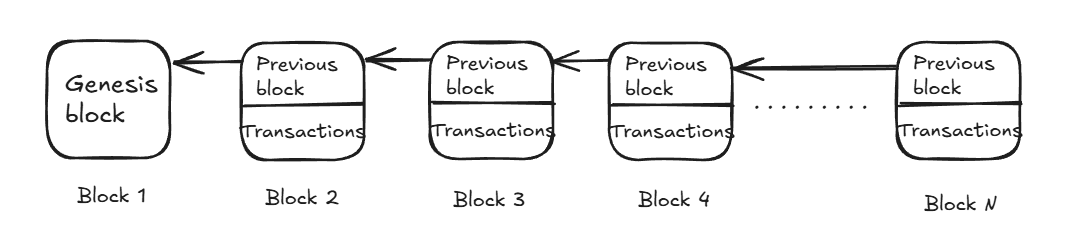
\includegraphics[width=0.7\textwidth]{imagenes/Estado del arte/estructuraDatosBlockchain.png}
    \caption{Representación gráfica de una blockchain. Fuente: \textcite{beginningBlockchain}}
    \label{fig:blockchain}
\end{figure}

Como se puede ver en la figura cada bloque esta compuesto por dos partes diferencias, el hash del bloque anterior y un conjunto de transacciones.
Se apunta al bloque anterior para garantizar que nadie pueda modificarlo sin alterar los bloques posteriores.

\subsection{Capas de la blockchain}
Según el libro \textcite{beginningBlockchain} la tecnología blockchain esta compuesta por varias capas:
\begin{itemize}
    \item \textbf{Capa de aplicación:} Es donde se programan las funciones que verá el usuario final. Se fomenta el uso de off-chain para cálculos o almacenamientos grandes y dejar la blockchain para lo esencial.
    \item \textbf{Capa de ejecución:} Aquí se ejecutan en todos los nodos las instrucciones definidas en la capa de aplicación: desde pasos simples hasta \textit{smart contracts}. Cada nodo (equipo participante en la red) ejecuta el programa de forma independiente.
    \item \textbf{Capa semántica:} Decide si las transacciones y bloques son válidos y en qué orden se insertan. Se definen reglas del sistema, modelos/estructuras de datos y se gestionan casos complejos vía smart contracts. También se define cómo los bloques se encadenan.
    \item \textbf{Capa de propagación:} Es la red P2P donde los nodos se comunican y sincronizan sobre el estado actual. Las transacciones y los bloques se difunden por toda la red para que todos conozcan el último bloque y puedan seguir construyendo encima. Por diseño un nodo reenvía lo nuevo a sus pares directos de inmediato. Puede haber latencias (segundos o más).
    \item \textbf{Capa de consenso:} Suele ser la base: su objetivo es que todos los nodos acuerden un mismo estado del libro mayor. Asegura la seguridad e integridad del sistema. El mecanismo concreto depende del caso de uso. Por ejemplo, en Ethereum se emplea Proof of Stake (PoS) para seleccionar el proponente de bloque y alcanzar finalidad; en Bitcoin se utiliza Proof of Work (PoW). Existen otros mecanismos, como dPoS o PBFT, según el tipo de red.
\end{itemize}    

\newpage
\section{Blockchain y su importancia en la logística} 
 Según \textcite{blockChainsForSupplChainManagement} La tecnología blockchain encaja a la perfección con la industria de la cadena de suministro, destacando elementos clave como la escalabilidad, el rendimiento, el mecanismo de consenso, la privacidad, la prueba de ubicación y los costos.
 Blockchain es una tecnología descentralizada, que permite hacer transacciones sin intermediarios de manera robusta y segura gracias a que una vez que los datos se han registrado en una cadena de blockchain, son inmutables.
 Esta tecnología encaja tan bien con la logística porque en el flujo de vida de un producto, desde que se fabrica hasta que es entregado, cada movimiento o cambio de etapa quedaría registrado mediante una transacción en la blockchain.

 \textbf{Principales ventajas de blockchain en este área}
 \begin{enumerate}
    \item Registrar cada activo individual desde productos hasta contenedores, a medida que va cambiando de etapa en la cadena de suministro.
    \item Rastrear órdenes, recibos, facturas, pagos y cualquier otro documento oficial de manera precisa y en tiempo real.
    \item Rastrear archivos digitales (como garantías, certificaciones, derechos de autor, licencias, números de serie y códigos de barras) de manera unificada y en paralelo con los activos físicos.
 \end{enumerate}
Además al ser una tecnología descentralizada contribuye eficientemente en la trazabilidad y al intercambio de información entre los distintos participantes.

\subsection{BlockTrack}
Habiendo descrito los problemas que hay en los sitemas actuales de gestión de la logística y la tecnología blockchain, se observa que sería interesante empezar a aplicar esta tecnología en las cadenas de suministro.
Gracias a blockchain, se incrementaría la confianza entre todas las partes involucradas, ya que tendrían acceso en tiempo real a toda la red, pudiendo consultar cualquier transacción relacionada con un producto de forma transparente y segura. Aclarar
que la tecnología blockchain no se limita solo a transacciones de dinero, sino que puede registrar cualquier tipo de información.

Además, cada nuevo bloque añadido a la red constituye información fiable y verificada, ya que debe ser validado mediante un mecanismo de consenso entre los nodos participantes. Al basarse en sistemas de seguridad como la criptografía de clave pública-privada y los hashes, se garantiza la integridad y la autenticidad de los datos.

Al tratarse de una red descentralizada, todas las transacciones se actualizan en tiempo real, lo que permite a todos los usuarios visualizar la información de forma consistente. Esto reduce las inconsistencias y mejora la eficiencia del sistema, ya que muchas de las verificaciones se eliminan al estar implícitas en el propio diseño de la tecnología blockchain.

Otra ventaja clave es que se detectarían errores en la cadena de suministro de un producto antes que los sistemas tradicionales gracias a la trazabilidad que brinda blockchain. Permitiendo a todos los usuarios acceder al historial completo de un producto en tiempo real. Esta visibilidad facilita solventar estos errores a edades más tempranas, reduciendo pérdidas económicas y mejorarando significativamente la experiencia de los clientes.

Por todas estas razones nace la idea de \textbf{BlockTrack}, esta aplicación se centrara en la etapa de transporte de la cadena de suministro de un producto, es decir comprenderá desde que un producto esta fabricado y empaquetado hasta que le llega al usuario final que podría ser un cliente u otra empresa. Cada movimiento
se añadirá a la blockchain mediante el uso de contratos inteligentes que ayudarán a automatizar estos procesos, permitiendo tanto a las empresas como a los usuarios siempre saber el estado del producto.

Esta aplicación tiene la idea de solventar por completo o parcialmente todos los problemas descritos de los sistemas tradicionales.
